\section*{\Large Task 2.5:}
Starting from the non-dimensional result obtained in the previous task, we can now obtain the dimensional results by multiplying the non-dimensional results by the characteristic scales of the problem, as follows:
\[
u_{dim} = u \cdot U_{\infty}, \qquad v_{dim} = v \cdot U_{\infty}, \qquad x_{dim} = x \cdot L, \qquad y_{dim} = y \cdot L
\]
assuming for $y$ the same characteristic scale of $x$.
To compute the carachteristic length $L$ we can use the formula: $Re_L = \frac{U_{\infty} L}{\nu}$
from which we get: $L = \frac{Re_L \cdot \nu}{U_{\infty}}$, and substituting the values of $Re_L = 10000$ and $\nu = 1.5 \times 10^{-5} \text{ m}^2/\text{s}$ we get $L = 0.0075 m$.

In conclusion the dimensional solution is reported in the following picture:
\begin{figure}[h]
  \centering
  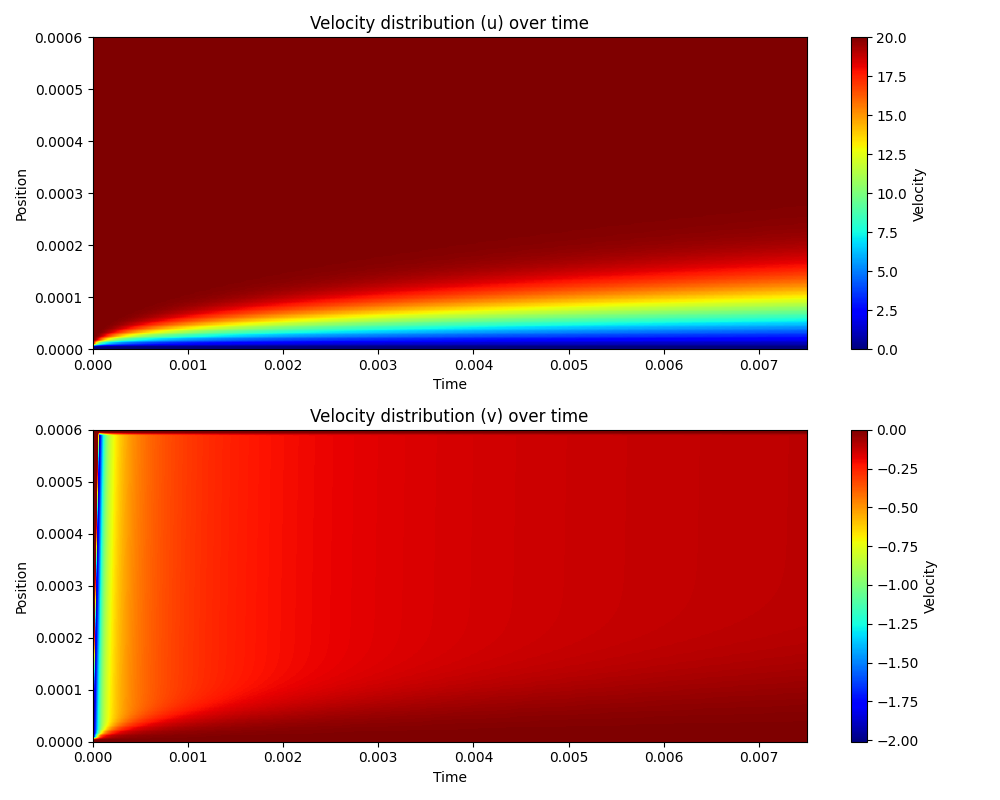
\includegraphics[width=0.5\textwidth]{result2.png}
  \caption{Dimensional solution}
\end{figure}

\section*{\Large Task 2.6:}
The stream function $\psi(x, y)$ is related to the velocity components as follows:

\begin{equation}
\frac{\partial \psi}{\partial y} = u, \qquad \frac{\partial \psi}{\partial x} = -v.
\end{equation}

To compute $\psi$ numerically, we integrate numerically over the spatial domain. We use a cumulative sum to integrate u along the y direction, imposing the boundary condition $\psi(0, y) = 0$.
The plot we get is the following:
\begin{figure}[h]
  \centering
  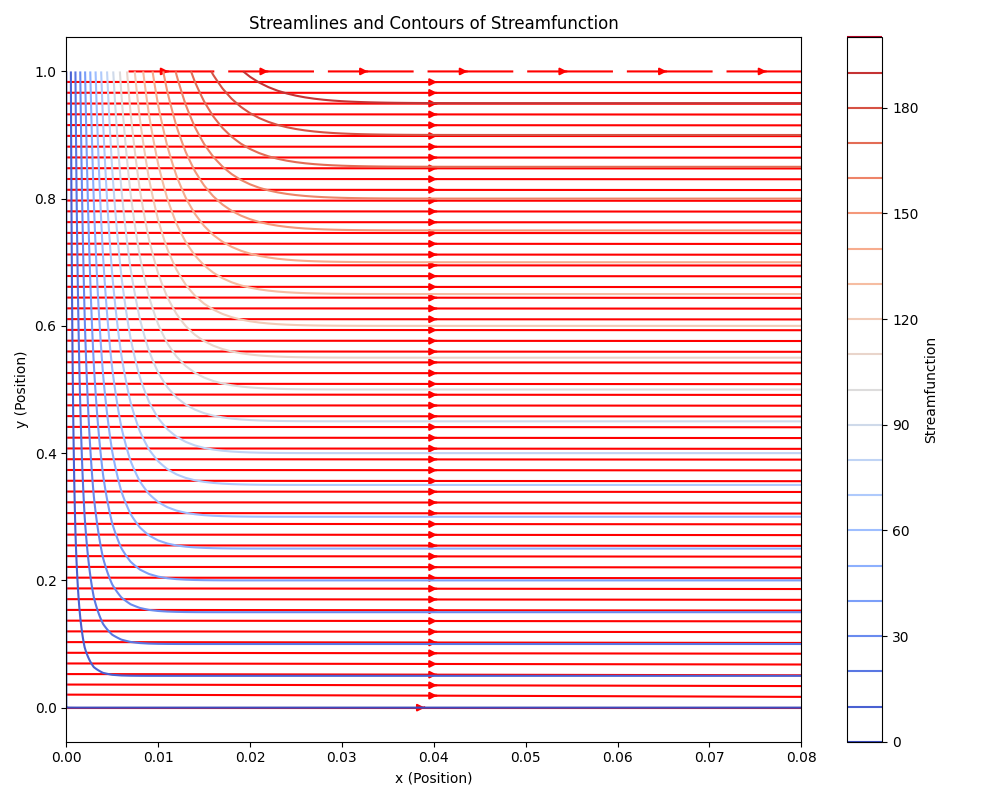
\includegraphics[width=0.5\textwidth]{task_2_6_fixed.png}
  \caption{Streamlines}
\end{figure}
The streamlines crossing the boundary layer edge indicate interaction between the external flow and the boundary layer. This can occur due to numerical errors in streamline calculation or physical effects like entrainment. If the boundary layer definition is well-resolved and no-slip conditions are enforced accurately, such behavior might suggest deviations in the streamline plot accuracy or physical flow features, depending on the resolution and method used.

\section*{\Large Task 2.7:}
The plots obtained by the code we implemented are shown in the following figures:
\begin{figure}[htbp]
\centering
\subfigure[Momentum thickness]{
  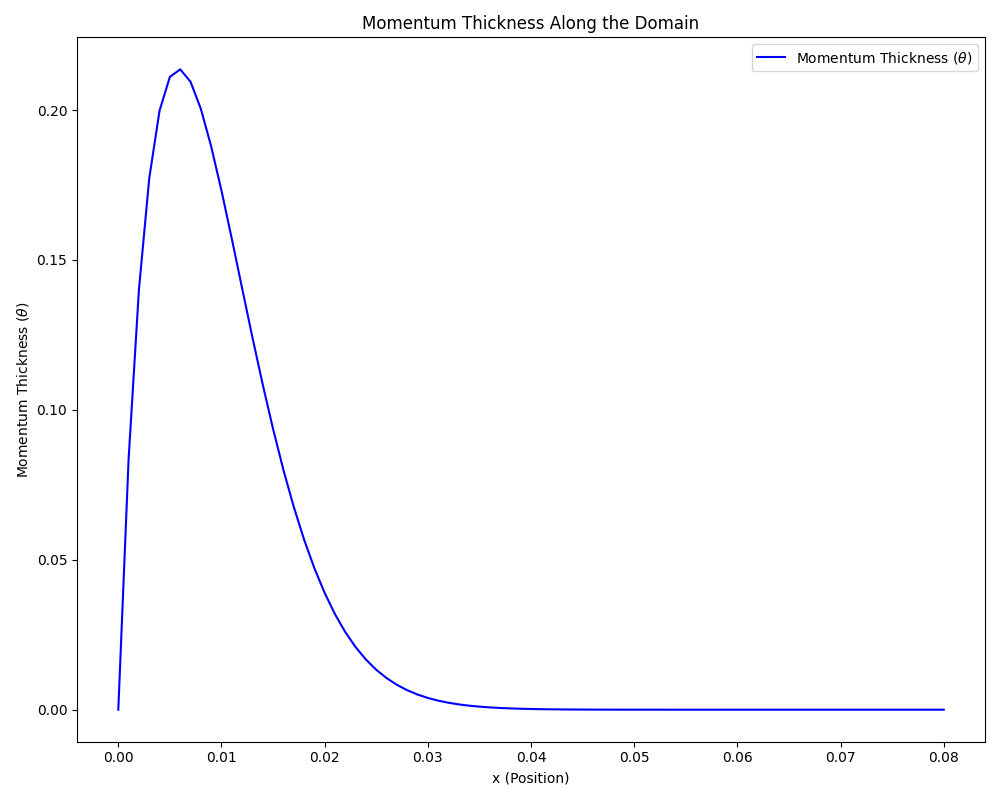
\includegraphics[width=0.45\textwidth]{task_2_7_momentum_thickness.png}
}
\hfill
\subfigure[Velocity profiles]{
  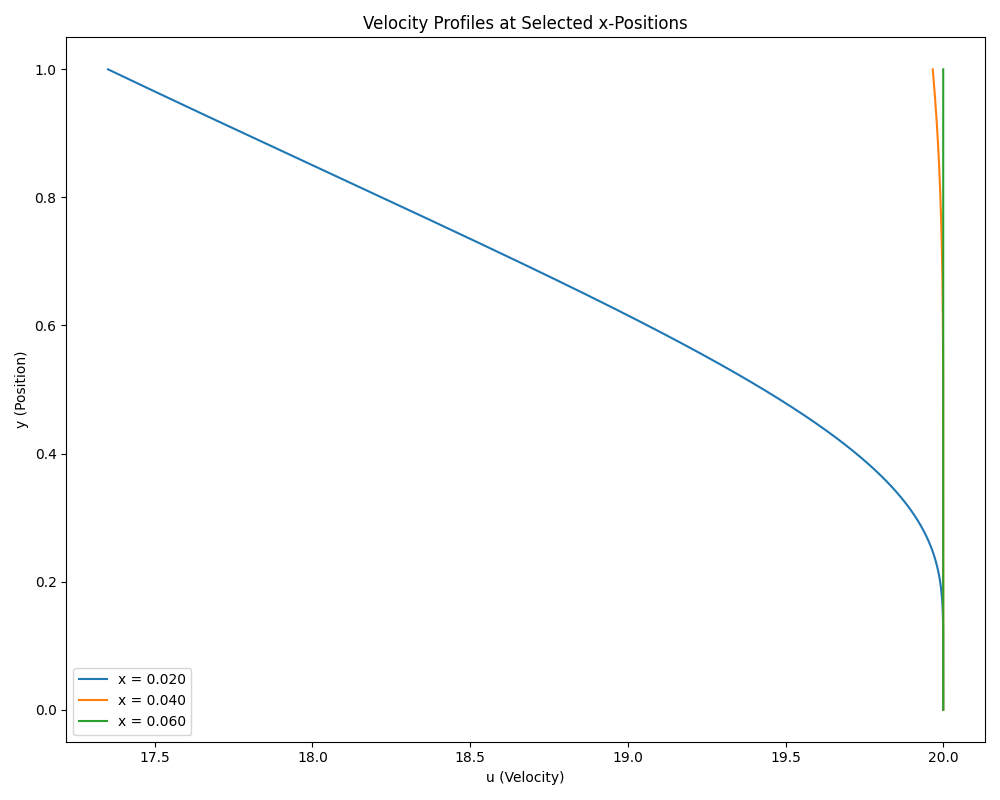
\includegraphics[width=0.45\textwidth]{task_2_7_velocity_profiles.png}
}
\label{fig:mieiduetrasparenti}
\end{figure}
Momentum thickness provides insight into the development of the boundary layer. It is a measure of the velocity distribution across the boundary layer and indicates how much momentum is being transported.
By plotting the momentum thickness along the domain, we can observe how it evolves with increasing $x$ (the streamwise position). Here we observe the typical behavior: momentum thickness increases initially as the boundary layer develops and then stabilizes as the flow becomes fully developed.

These profiles allow us to analyze the shape of the boundary layer at different streamwise locations. At lower $x$-values (near the leading edge), the profiles are steeper, indicating that the boundary layer is still developing.
As $x$ increases, the profiles tend to become more gradual, representing the fully developed boundary layer.

Streamlines represent the actual flow trajectories of fluid particles, showing the path the fluid takes under the influence of the velocity field. They indicate the direction of flow and provide insights into the flow patterns like vortices or separation.
Iso-lines of the streamfunction epresent regions of constant flow and are mathematically derived from the velocity field. They indicate the same flow features but are typically smoother and more evenly spaced in a well-behaved flow.

Considering their meaning we expect to generally coincide, as both describe the same physical flow. However, differences might appear due to numerical errors, interpolation methods, or grid resolution, especially in regions with complex flow patterns or sharp gradients.
In particular in this case we were not able to print them due to some issues in the code.
